
\chapter{Getting started}

Once you have installed your Corina Desktop application and you have access to a Corina server you are now ready to launch Corina for the first time.

\section{First time launch}

When you launch Corina you will be presented with a dialog (figure \ref{fig:login}) for logging in to your the Corina webservice.

\begin{wrapfigure}{r}{0.5\textwidth}
  \begin{center}
    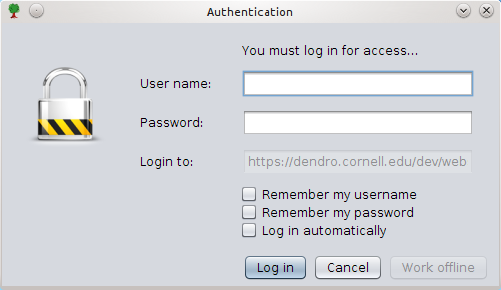
\includegraphics[width=0.48\textwidth]{Images/login.png}
  \end{center}
  \caption{Corina webservice login dialog.}
  \label{fig:login}
\end{wrapfigure}

You must fill in the `Login to' field with the URL of the Corina webservice that you would like to connect to.  This should have been provided to you by your Corina systems administrator (if you are using a centralized lab database) otherwise if you are using a Corina Virtual Appliance it can be obtained from your Corina command line (see the Virtual Appliance installation instructions on page \pageref{txt:virtualAppliance}).  The username and password are your Corina login credentials (not your system or network credentials) provided to you by your systems administrator.  Details of the default administrator credentials for Virtual Appliance users are also provided on page \pageref{txt:virtualAppliance}.  The dialog gives you the option for saving your username and/or password if you prefer.  We recommend using this feature only on personal machines.  You may choose to cancel the login if you like and Corina will continue to load, however, you will not have access to the Corina database therefore very few functions will be available to you.

Once you have logged in you will be presented with the Corina home screen.  This contains the main menus for the program as well as three quick-link icons for creating new records, opening existing records and importing existing data files to the database.


\section{Configuring measuring platforms}
\index{Measuring platforms}
\index{Hardware|see{Measuring platforms}}

Although it is possible to manually enter the ring widths of your samples into Corina, it is normal to automate this process using a measuring platform. Corina supports the most common measuring platforms including Velmex and Lintab.  However, please note that standard Lintab platforms use a proprietary communications protocol. Rinntech--the manufacturers of Lintab platforms--claim intellectual property rights over this protocol. During discussions between the Corina development team and Rinntech an agreement was reached whereby the Corina developers agreed not to release details of the protocol. In turn Rinntech has agreed to produce an adapter that can be attached to Lintab platforms so that they communicate with an open ASCII protocol. Users wishing to use Lintab platforms with Corina (or any software not developed by Rinntech) must therefore contact Rinntech and purchase an adapter.

Measuring platforms typically use serial ports to communicate to computers. In recent years computer manufacturers have been phasing out serial ports so you may need to purchase a serial-USB converter. Modern MacOSX, Linux as well as Windows 7 should support most serial-USB adapters out of the box, otherwise you must install the relevant drivers before continuing.  Recent Lintab USB platforms use internal serial-USB converters so are treated in exactly the same way by Corina.

To begin, shut down your computer, attach your platform, then reboot and launch Corina. Next, go to the preferences window and open the hardware tab and you should see an interface that looks like figure \ref{fig:hardwareprefs}.

\begin{figure}[hbtp]
  \centering
    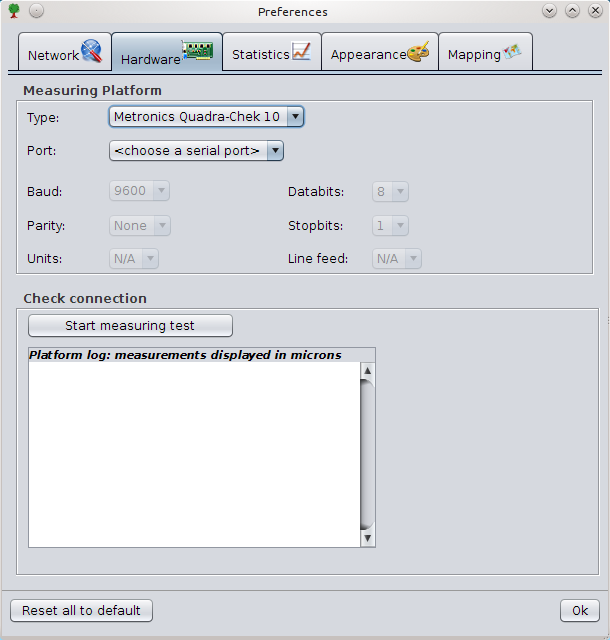
\includegraphics[width=0.6\textwidth]{Images/hardwareprefs.png}
    \caption{The hardware preferences dialog.}
    \label{fig:hardwareprefs}
\end{figure}

In the type pull down menu, select the type of measuring equipment you are using. Note that this refers to the equipment that the computer is attached to, and not necessarily the measuring platform itself. For instance, Velmex platforms are typically connected through a Metronics digital readout device. Included in this list is the EveIO device which is an open-source device designed for the Cornell Tree-Ring Laboratory. Circuit drawings for this device can be obtained from the Cornell lab to enable Hensen measuring platforms to be used with Corina (and other software).

Next you must choose the port that your platform is connected to from the pull down menu. In Windows this will be a COM port, in Linux and Mac this will be a /dev/xxx port.  Depending on the type of platform you choose, you may also need to set various communication parameters.  If these boxes are enabled, please check the documentation that came with your measuring platform to ensure these values are set correctly.

To check whether your platform is working, click the `Start measuring test' button and attempt to measure a few rings.  Once you are satisfied, click OK on the preferences window and you will be returned to the Corina home screen.

Different measuring platforms have different capabilities.  For instance, some include a physical switch for firing measurement events, others also include switches for resetting measurements to zero.  Some platforms (e.g. Lintab) also continuously report the measurement values to the computer.  So depending on the hardware you use, Corina will present the you with slightly different options.  

Please note that the architecture of Corina is such that providing support for additional measuring platforms is a relatively simple task.  If you have equipment that is not currently supported, please contact the developers to see if it can be included.  


\section{Measuring a new sample}
\index{Sample!Measuring|(}
Once your measuring platform has been configured, measuring your first sample is simple.  To start a new measurement go to \menutwo{File}{New} or click the `new' icon on the home screen. A dialog will appear where you can scan your sample's barcode, or press the button to enter metadata for your sample later. Barcodes minimize data entry errors and also speed up the process of measuring your samples. See section \ref{txt:barcodes} for more information. Once you have scanned your barcode or pressed the button, you will then be presented with an empty Corina data screen (figure \ref{fig:datascreen}).

\begin{figure}[hbtp]
  \centering
    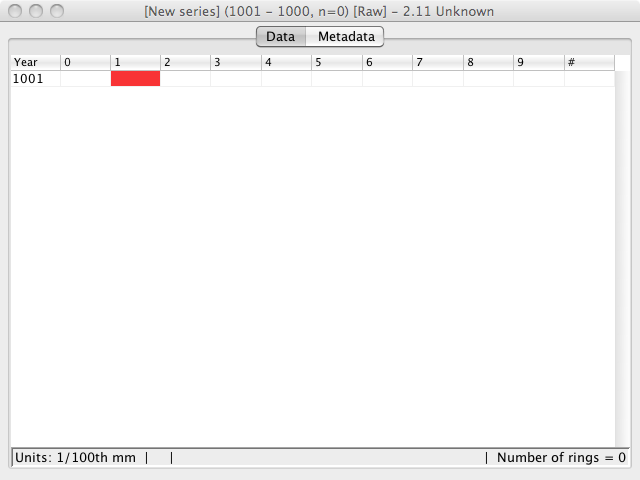
\includegraphics[width=0.6\textwidth]{Images/datascreen.png}
    \caption{An empty data window ready to receive measurements.  Note the status bar at the bottom includes buttons for changing the display units and cumulative statistics.}
    \label{fig:datascreen}
\end{figure}

The next step is to fill out the metadata tab. If you have used a barcode, nearly all of this metadata will be filled in for you, otherwise you will need to fill this out yourself. Details about metadata can be found in chapter \ref{txt:metadata}, page \pageref{txt:metadata}.

To begin measuring your sample you can now go to \menutwo{Edit}{Start measuring} or you can press F5. While measuring you should be provided with audible feedback for each ring measured with a more pronounced sound made every 10th ring. If there is a problem communicating with your measuring hardware, check your settings in the preferences dialog. If you still have problems contact the Corina developers by going to \menutwo{Help}{Report bug on last transaction}, making sure you include your email address and any further information.


\index{Ring remarks}
While you measure your sample you can flag features in a ring by right clicking on any cell in the table and selecting one or more of the standard notes (see figure \ref{fig:ringremarks}).

Corina supports all standard TRiDaS remarks including: fire damage; frost damage; crack; false ring(s); compression wood; tension wood; traumatic ducts; single pinned; double pinned; triple pinned and many others.  Rings that include remarks are indicated by the relevant icon in the data screen.  Depending on your method of work, this can be useful for keeping track of sample pin holes.  For instance, if a missing or false ring is discovered after a sample has been pinholed, the offset in pinholes can be easily seen without resurfacing the sample.  In the future Corina will also include support for user defined ring remarks.  

\begin{wrapfigure}{r}{0.5\textwidth}
  \begin{center}
    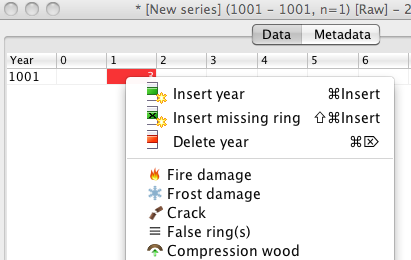
\includegraphics[width=0.42\textwidth]{Images/ringremarks.png}
  \end{center}
  \caption{Right click context menu showing some of the options for adding remarks to rings.}
  \label{fig:ringremarks}
\end{wrapfigure}

The data screen also contains a status bar at the bottom. By click on the units section, you can switch between micron and 1/100th mm units. Corina understands the units being supplied by the measuring platform, therefore changes here are purely for display purposes only. If you have a platform that measures in microns, but prefer to see the values in 1/100th mm then you can use this feature. At the bottom ring of the status bar you can choose one of a variety of summary information about your series.

Once you have finished measuring your sample, you should then go to \menutwo{File}{Save} to save your series to the database. 
\index{Sample!Measuring|)}


\section{Opening existing data}
\index{Sample!Opening}
If you have used traditional dendrochronology software, you are probably used to opening existing dendro data files from your computer.  Corina works in a different way.  All data accessed by Corina is stored within the central Corina database rather than from files.  The database provides many benefits over file based storage, most importantly it means there is a high degree of security and integrity in your data.  

To use data that you have stored in existing data files you must first \emph{import} your data into the Corina database.  This gives you the opportunity to clean-up your data!  For details of how to import your data see chapter \ref{txt:importExport}, page \pageref{txt:importExport}.

Once you have data in your database, either by importing existing data files or measuring new samples, you can access your data through the database browser.  This is accessed through the \menutwo{File}{Open} or \menutwo{File}{Open multiple} menus and an example of the dialog is shown in figure \ref{fig:dbbrowser}. The same database browser dialog is used in multiple places throughout Corina, e.g.\ when adding addition series to graphs and when choosing chronologies to crossdate against. 

\begin{figure}[hbtp]
  \centering
    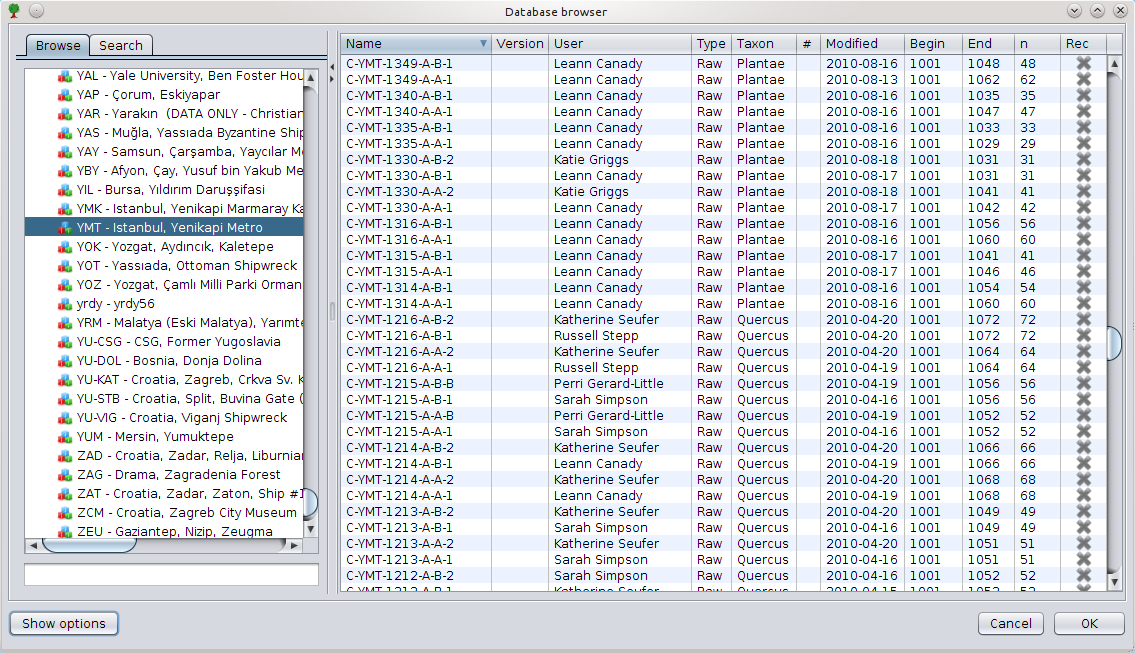
\includegraphics[width=0.9\textwidth]{Images/dbbrowser.png}
    \caption{Screenshot of the database browser dialog.}
    \label{fig:dbbrowser}
\end{figure}

The database browser is divided into two main parts.  On the left is the browse and search tabs, and on the right is the series table.  Selecting options in the browse or search tab populates the series table on the right with all the series that match the specified criteria.  

\warn{The search tab is currently a `work-in-progress' so we recommend you use the browse tab until further notice.}

The browse tab shows a heirarchical tree view of the contents of your Corina database based upon the TRiDaS data model.  The panel will be pre-populated with all the objects in your database but it is possible to `drill-down' by right clicking on an object and choosing `Expand branch'.  Expanding an object for instance, will show all the elements associated with that object, and expanding an element will show all the samples associated with the specified element.  To better understand the TRiDaS terminology please read chapter \ref{txt:metadata}, page \pageref{txt:metadata}.

By double clicking (or right clicking and choosing `Search for associated series') on an item in the browse panel Corina will search the database for all series that are associated with the specified entity.  The results of the search will be shown in the series table on the right of the screen.  This table shows basic metadata about each search and is sortable by click on any of the column headers.  To open a series, simply select one of these series and click `OK'.  If the database browser is open in 'multiple series' mode, then you can use the arrow buttons to select multiple series to open in one go.

There is also a `Show options' button on the database browser dialog.  This adds additional advanced methods for filtering the series table to help you find the data you are interested in.

\section{Reconciling data}
\index{Sample!Reconciling}
Corina has been developed not only for experience dendrochronologists, but as a tool for teaching students.  It therefore includes a comprehensive `reconciling' tool for supervisors to check the quality of measurements made by students.  The reconcile dialog does a comparison of a measurement series made by a student with a references series of the same radius measured by the supervisor.  The same dialog can also prove useful for comparing measurements from two experienced dendrochronologists when handling particularly difficult samples.

 


